\section{Introduction}
\label{sec:intro}
The search for Higgs boson production in association with a top quark pair (ttH) in the $\mathrm{H\rightarrow bb}$~\cite{HIGG-2017-03} and $\mathrm{H\rightarrow}$ multi-lepton~\cite{ATLAS-CONF-2019-045} final states is limited by the modelling uncertainties of the main backgrounds, tt+bb and tt+V respectively, where V denotes either a W or Z boson. Examples of tree-level diagrams of said processes are shown in Figure~\ref{intro:sig}. A comparison of available Monte Carlo generators is thus performed to study modelling differences. Comparisons of observables are made at particle level, in a phase space similar to the reference measurements. Differences in the object and event selection were made to define a common selection with the CMS collaboration, to later compare these distributions between the two experiments. The goal is to decide on a common strategy between ATLAS and CMS for background modelling uncertainties in the ttH(bb) and ttH(multi-lepton) analyses.

\begin{figure}[!htb]
\centering

\includegraphics[width=0.35\textwidth]{Plots/ttbb/ttbb}
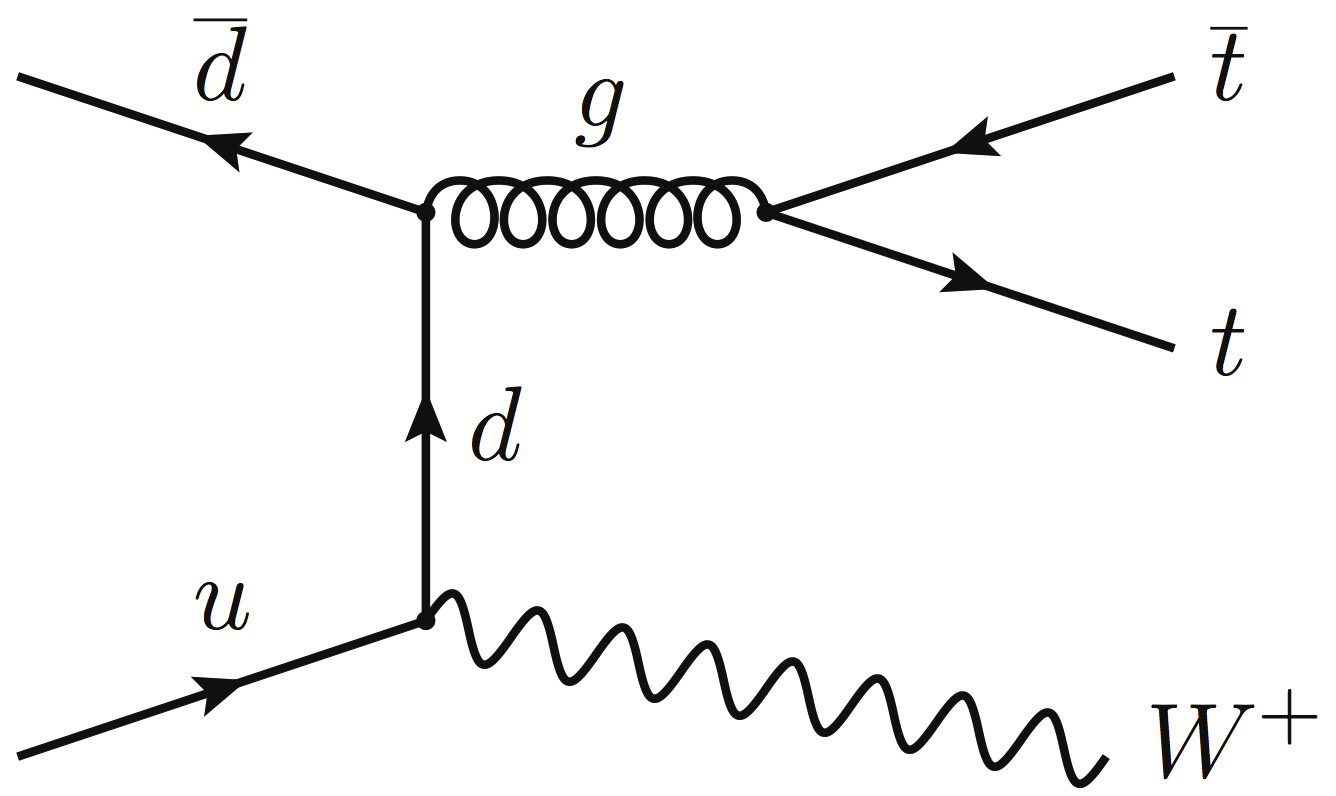
\includegraphics[width=0.35\textwidth]{Plots/ttV/ttW}
  \caption{Examples of tree-level Feynman diagrams for tt+bb (left) and tt+W (right). \label{intro:sig}}
\end{figure}